%%%%%%%%%%%%%%%%%%%%%%%%%%%%%%%%%%%%%%%%%
% Lachaise Assignment
% LaTeX Template
% Version 1.0 (26/6/2018)
%
% This template originates from:
% http://www.LaTeXTemplates.com
%
% Authors:
% Marion Lachaise & François Févotte
% Vel (vel@LaTeXTemplates.com)
%
% License:
% CC BY-NC-SA 3.0 (http://creativecommons.org/licenses/by-nc-sa/3.0/)
% 
%%%%%%%%%%%%%%%%%%%%%%%%%%%%%%%%%%%%%%%%%

%----------------------------------------------------------------------------------------
%	PACKAGES AND OTHER DOCUMENT CONFIGURATIONS
%----------------------------------------------------------------------------------------

\documentclass{article}
\usepackage{float}
%%%%%%%%%%%%%%%%%%%%%%%%%%%%%%%%%%%%%%%%%
% Lachaise Assignment
% Structure Specification File
% Version 1.0 (26/6/2018)
%
% This template originates from:
% http://www.LaTeXTemplates.com
%
% Authors:
% Marion Lachaise & François Févotte
% Vel (vel@LaTeXTemplates.com)
%
% License:
% CC BY-NC-SA 3.0 (http://creativecommons.org/licenses/by-nc-sa/3.0/)
% 
%%%%%%%%%%%%%%%%%%%%%%%%%%%%%%%%%%%%%%%%%

%----------------------------------------------------------------------------------------
%	PACKAGES AND OTHER DOCUMENT CONFIGURATIONS
%----------------------------------------------------------------------------------------

\usepackage{amsmath,amsfonts,stmaryrd,amssymb} % Math packages

\usepackage{enumerate} % Custom item numbers for enumerations

\usepackage[ruled]{algorithm2e} % Algorithms

\usepackage[framemethod=tikz]{mdframed} % Allows defining custom boxed/framed environments

\usepackage{listings} % File listings, with syntax highlighting
\lstset{language=C,keywordstyle={\bfseries \color{blue}}}

%----------------------------------------------------------------------------------------
%	DOCUMENT MARGINS
%----------------------------------------------------------------------------------------

\usepackage{geometry} % Required for adjusting page dimensions and margins

\geometry{
	paper=a4paper, % Paper size, change to letterpaper for US letter size
	top=2.5cm, % Top margin
	bottom=3cm, % Bottom margin
	left=2.5cm, % Left margin
	right=2.5cm, % Right margin
	headheight=14pt, % Header height
	footskip=1.5cm, % Space from the bottom margin to the baseline of the footer
	headsep=1.2cm, % Space from the top margin to the baseline of the header
	%showframe, % Uncomment to show how the type block is set on the page
}

%----------------------------------------------------------------------------------------
%	FONTS
%----------------------------------------------------------------------------------------

\usepackage[utf8]{inputenc} % Required for inputting international characters
\usepackage[T1]{fontenc} % Output font encoding for international characters

\usepackage{XCharter} % Use the XCharter fonts

%----------------------------------------------------------------------------------------
%	COMMAND LINE ENVIRONMENT
%----------------------------------------------------------------------------------------

% Usage:
% \begin{commandline}
%	\begin{verbatim}
%		$ ls
%		
%		Applications	Desktop	...
%	\end{verbatim}
% \end{commandline}

\mdfdefinestyle{commandline}{
	leftmargin=10pt,
	rightmargin=10pt,
	innerleftmargin=15pt,
	middlelinecolor=black!50!white,
	middlelinewidth=2pt,
	frametitlerule=false,
	backgroundcolor=black!5!white,
	frametitle={Command Line},
	frametitlefont={\normalfont\sffamily\color{white}\hspace{-1em}},
	frametitlebackgroundcolor=black!50!white,
	nobreak,
}

% Define a custom environment for command-line snapshots
\newenvironment{commandline}{
	\medskip
	\begin{mdframed}[style=commandline]
}{
	\end{mdframed}
	\medskip
}

%----------------------------------------------------------------------------------------
%	FILE CONTENTS ENVIRONMENT
%----------------------------------------------------------------------------------------

% Usage:
% \begin{file}[optional filename, defaults to "File"]
%	File contents, for example, with a listings environment
% \end{file}

\mdfdefinestyle{file}{
	innertopmargin=1.6\baselineskip,
	innerbottommargin=0.8\baselineskip,
	topline=false, bottomline=false,
	leftline=false, rightline=false,
	leftmargin=2cm,
	rightmargin=2cm,
	singleextra={%
		\draw[fill=black!10!white](P)++(0,-1.2em)rectangle(P-|O);
		\node[anchor=north west]
		at(P-|O){\ttfamily\mdfilename};
		%
		\def\l{3em}
		\draw(O-|P)++(-\l,0)--++(\l,\l)--(P)--(P-|O)--(O)--cycle;
		\draw(O-|P)++(-\l,0)--++(0,\l)--++(\l,0);
	},
	nobreak,
}

% Define a custom environment for file contents
\newenvironment{file}[1][File]{ % Set the default filename to "File"
	\medskip
	\newcommand{\mdfilename}{#1}
	\begin{mdframed}[style=file]
}{
	\end{mdframed}
	\medskip
}

%----------------------------------------------------------------------------------------
%	NUMBERED QUESTIONS ENVIRONMENT
%----------------------------------------------------------------------------------------

% Usage:
% \begin{question}[optional title]
%	Question contents
% \end{question}

\mdfdefinestyle{question}{
	innertopmargin=1.2\baselineskip,
	innerbottommargin=0.8\baselineskip,
	roundcorner=5pt,
	nobreak,
	singleextra={%
		\draw(P-|O)node[xshift=1em,anchor=west,fill=white,draw,rounded corners=5pt]{%
		Question \theQuestion\questionTitle};
	},
}

\newcounter{Question} % Stores the current question number that gets iterated with each new question

% Define a custom environment for numbered questions
\newenvironment{question}[1][\unskip]{
	\bigskip
	\stepcounter{Question}
	\newcommand{\questionTitle}{~#1}
	\begin{mdframed}[style=question]
}{
	\end{mdframed}
	\medskip
}

%----------------------------------------------------------------------------------------
%	WARNING TEXT ENVIRONMENT
%----------------------------------------------------------------------------------------

% Usage:
% \begin{warn}[optional title, defaults to "Warning:"]
%	Contents
% \end{warn}

\mdfdefinestyle{warning}{
	topline=false, bottomline=false,
	leftline=false, rightline=false,
	nobreak,
	singleextra={%
		\draw(P-|O)++(-0.5em,0)node(tmp1){};
		\draw(P-|O)++(0.5em,0)node(tmp2){};
		\fill[black,rotate around={45:(P-|O)}](tmp1)rectangle(tmp2);
		\node at(P-|O){\color{white}\scriptsize\bf !};
		\draw[very thick](P-|O)++(0,-1em)--(O);%--(O-|P);
	}
}

% Define a custom environment for warning text
\newenvironment{warn}[1][Warning:]{ % Set the default warning to "Warning:"
	\medskip
	\begin{mdframed}[style=warning]
		\noindent{\textbf{#1}}
}{
	\end{mdframed}
}

%----------------------------------------------------------------------------------------
%	INFORMATION ENVIRONMENT
%----------------------------------------------------------------------------------------

% Usage:
% \begin{info}[optional title, defaults to "Info:"]
% 	contents
% 	\end{info}

\mdfdefinestyle{info}{%
	topline=false, bottomline=false,
	leftline=false, rightline=false,
	nobreak,
	singleextra={%
		\fill[black](P-|O)circle[radius=0.4em];
		\node at(P-|O){\color{white}\scriptsize\bf i};
		\draw[very thick](P-|O)++(0,-0.8em)--(O);%--(O-|P);
	}
}

% Define a custom environment for information
\newenvironment{info}[1][Info:]{ % Set the default title to "Info:"
	\medskip
	\begin{mdframed}[style=info]
		\noindent{\textbf{#1}}
}{
	\end{mdframed}
} % Include the file specifying the document structure and custom commands

%----------------------------------------------------------------------------------------
%	ASSIGNMENT INFORMATION
%----------------------------------------------------------------------------------------

\title{CS426: Project \#3 Report} % Title of the assignment

\author{Doruk Çakmakçı\\ \texttt{21502293}} % Author name and email address

\date{Bilkent University --- \today} % University, school and/or department name(s) and a date

%----------------------------------------------------------------------------------------

\begin{document}

\maketitle % Print the title

%----------------------------------------------------------------------------------------
%	INTRODUCTION
%----------------------------------------------------------------------------------------

\section{Description of Profiling Outputs Using gprof} 
\qquad For this project, code profiling is done in order to find what constitutes most to the running time of both the sequential and the parallel implementations. The gprof tool is used for profiling both implementations. The gprof tool is used as the following: First, the source code is compiled using -pg flag which produces gmon.out file which is used later on. Then, the executable produced from the compilation process is run using the necessary inputs to produce information that will be profiled. Finally using the gprof command, the produced executable and gmon.out file, the code profile is dumped to a text file(For this project, the resulting files are prof\_sequential.txt and prof\_omp.txt). In the profiling outputs, verbose information are omitted using -b flag to produce a nice output.\\
\null \qquad The output of gprof tool consists of the following components: 
\begin{itemize}
    \item \textbf{Flat Profile} consists of the information about how the total running time of the program is distributed to specific functions(e.g. distribution of timing to execution of functions) without considering the callee functions inside a function. Flat Profile has the following fields:
        \begin{itemize}
            \item \textbf{\%(in time units)} gives the percentage in terms of the total running time of the program spent in the function.
            \item \textbf{cumulative(in milliseconds)} is the running sum of the number of seconds accounted seconds for by this function and those listed above it.
            \item \textbf{self(in milliseconds)} is the number of seconds accounted for by this seconds function alone.
            \item \textbf{calls} is the number of times this function is called.
            \item \textbf{self(in milliseconds per call)} is the average number of milliseconds spent per call of the function 
            \item \textbf{total(in milliseconds per call)} is the average number of milliseconds spent per call of the function and its descendants per call
            \item \textbf{name} is the name of the function.
        \end{itemize}   
    \item \textbf{Call Graph} describes the call tree of the program, and it is sorted with respect to the total amount of time spent in each function and its children. Call Graph has the following fields: 
        \begin{itemize}
            \item \textbf{index} is a unique identifier of the functions that combine to generate the total time. The lowest index is given to the most time consuming(Aggregate time that is generated by the function and the callee functions) function and the highest index is given to the minimum time consuming function(and called functions). 
            \item \textbf{\%time} gives how much the function under consideration and the called functions inside this function contributes to the total timing in terms of percentage.
            \item \textbf{self} shows how much time the function spends without taking the time of the callee functions.
            \item \textbf{children} field lists the total amount of time propagated into this function by its children.
            \item \textbf{called} field gives the number of times the function was called and lastly, name field gives the name of the function.
        \end{itemize}   
\end{itemize}

\section{Description of Implementation Details}
\qquad First, the following pragmas are used during implementation:
\begin{itemize}
    \item \textbf{\#pragma omp parallel for} is used to make a insert a parallel region around the for loop that is paralelized. Also provides an implicit barrier for thread syncronization at the end of the loop. To disable the implicit barrier, a nowait clause should be used within for loop. The loop index variable is implicitly made private to the thread. Also, clasuses such as single, atomic, critical, if, schedule, num\_threads and much more clauses can be used in the scope of this pragma. Also, private, shared, default, firstprivate and lastprivate clauses can be used for declaring variable scopes.
    \item \textbf{\#pragma omp atomic} can only be used for statements that are wanted to be atomically executed by the threads. In other words, it provides a critical region around the statement for which it is used.
    \item \textbf{\#pragma omp critical} is used where only one thread must be executing a code segment at one time. When used, in the critical region, always 1 thread will be executing concurrently. This directive can be used with named critical region or unnamed critical region. Also, if option can be used to 
\end{itemize}
\qquad  In the following discussion, the parallelized segments are identified by the job they do and the line numbers in lbp\_omp.c file. The sequential implementation is parallelized using OpenMP. Accoridng to profiling results of the sequential implementation, create\_histogram and distance function should be parallelized. But further parallelism is also done to the implementation. First in create\_histogram function, the following parallelisms are done:
\begin{itemize}
    \item \textbf{Line 13-16:} The elements of the hist parameter should be initialized to 0. Although this parallelism is not necessary, the for loop that initializes elements of hist array is parallelized using "\#pragma omp parallel for" directive. With this directive any option available for "parallel" directive can be used. To be exact, the following options could be used: shared, private, default, firstprivate, lastprivate. Since this is a parallelism that is not essential to solve for the bottleneck, only the shared option is used on hist variable since all threads do mutually exclusive job on setting the elements of hist array(there is no race condition) and we need the updated elements of hist array.
    \item \textbf{Local Binary Pattern Analysis} As defined in the project documentation, local binary pattern analysis should be done on the pixels of the image. This analysis is divided to interior pixels, border pixels and edge pixels. These lines do the interior pixel analysis. The local binary pattern analysis is one of the main bottlenecks of the sequential implementation so these line segments are parallelized. Further discussion of these line segments are below:
    \begin{itemize}
        \item \textbf{Line 22-48(Interior Pixels):} In order to parallelize this segment "\#pragma omp parallel for" directive is used. The options available for this pragma are default, share, private, firstprivate and lastprivate. There also may be more advanced options for this pragma but the listed ones are enough for many applications. For this segment, I used private, shared and default options. Also, since the value of hist[index] must be updated in a mutually exclusive manner to eliminate race conditions between threads working in this parallel region, "\#pragma omp atomic" directive is used. Instead of atomic, a critical region may be used to ensure atomic increment operation by using "\#pragma omp critical" directive.
        \item \textbf{Line 53-75, 77-99, 101-123, 125-147(Border Pixels):} In like manner with the analysis for Interior pixels, "\#pragma omp parallel for" and "\#pragma omp atomic" directives were used for the same use cases.
        \item \textbf{Line 152-236(Edge Pixels):} The same operation is done for the 4 edge pixels, the pixels are processed in a sequential manner, similar to an unrolled loop.
    \end{itemize}
\end{itemize}
\null \qquad Then, distance function(Line 239-259) is parallelized. There is a for loop for all elements of the input arrays, the loop is parallelized using "\#pragma omp parallel for" directive and with private, shared and default clauses. In this for loop, distance variable must be updated mutually exclusively by threads so the updates to distance variable is done in a critical region. Critical region is declared unnamed. Also, instead of critical region, a reduction on the running variable may also be implemented as an alternative to the critical region. \\
\null \qquad Then, find\_closest function is parallelized. The for loop for processing training set images is processed since it is a bottleneck to the sequential implementation. The for loop is parallelized using "#pragma omp parallel for" directive with private, shared and default clauses. Also, since minimum\_distance variable must be updated mutually exclusively to eliminate race conditions, the updates to min\_dist variable are surrounded with an unnamed critical region without any clauses. \\
\null \qquad Finally, some parts of the main program is parallelized. The allocation of the 2D matrices to hold histograms is done in a for loop. This fpor loop is parallelized using "#pragma omp parallel for" directive with shared, private and default clauses since the operation done in the loop is mamory allocation. Then, the creation of the histograms for training images and test images is critical for decreasing the program running time. The for loops for generating the histograms are parallelized using "\#pragma omp parallel for" directives with private, shared and default clauses.

\section{Results}
\subsection{Accuracy vs K}
\begin{figure}[H]
\centering
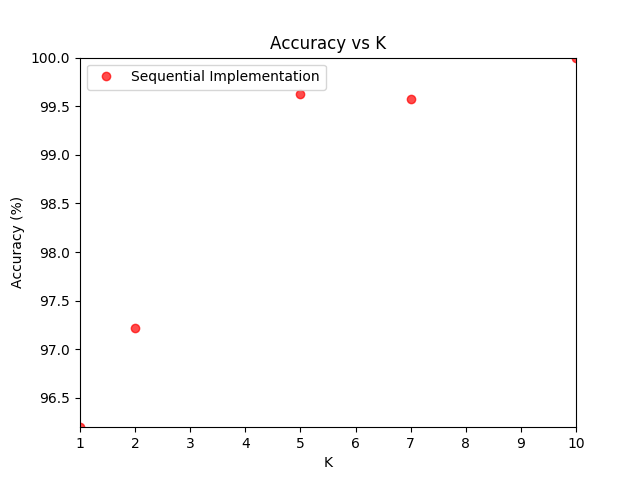
\includegraphics[width=\linewidth]{assets/acc_vs_K_sequential.png}
\label{fig:test1}
\vspace{-2pt}
\caption{Accuracy vs. K value for sequential implementation}
\end{figure}
\begin{figure}[H]
\centering
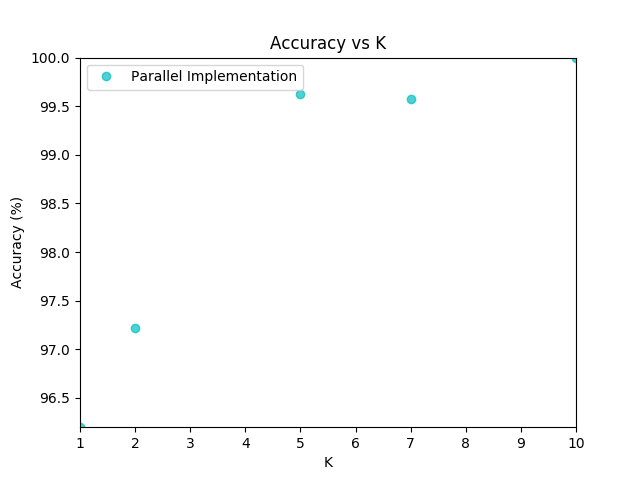
\includegraphics[width=\linewidth]{assets/acc_vs_K_parallel.png}
\label{fig:test1}
\vspace{-2pt}
\caption{Accuracy vs. K value for parallel implementation}
\end{figure}

\subsubsection{Discussion}
\qquad The parallel and sequential implementation must not differ in terms of accuracy for same K value since this project is based on a static problem and the results are not time varying. We see that the results of parallel and sequential execution are same. Naturally, we see the accuracy is increasing with K value. This is due to increased number of training examples to base the prediction of test examples. However, the accuracy of K = 7 is less than  K = 5. This is due to presence of outliers for each person's images. Mainly, the 20 images belonging to a person must have similar characteristics from a perspective but it seems that there exists an outlier in the images of a person.


\subsection{Execution Time vs Number of Threads}
\begin{figure}[H]
\centering
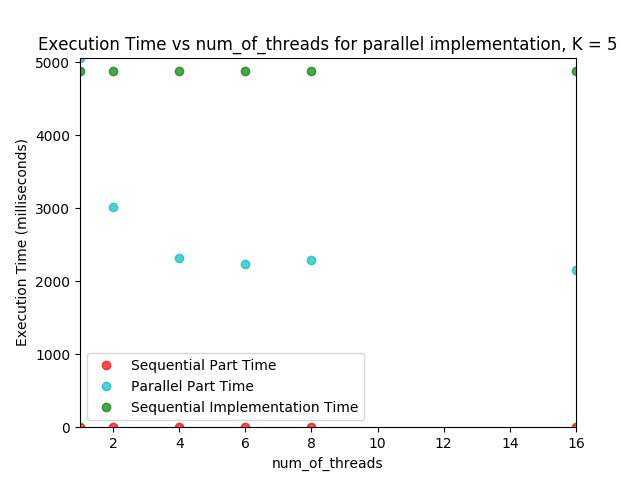
\includegraphics[width=\linewidth]{assets/time_vs_num_of_threads_parallel_K_5.png}
\label{fig:test1}
\vspace{-2pt}
\caption{Execution time vs num\_of\_threads for parallel implementation. K is set to 5.}
\end{figure}
\subsubsection{Discussion}
\qquad As seen from the plot, as the number of threads increase linearly, parallel running times decrease in exponential manner with diminishing returns. After num\_of\_threads is increased beyond 4, the threads can not be utilized as much. The utilization of threads is dependent to the value of computation per thread. We can infer that adding more threads not always decrease runtime of a program. The optimal number of threads is dependent to the amount of paralelism and the nature of the problem.\\
\null \qquad We see that sequential part time is always 0. This is because printing is done in the scope of parallel time computation even though printing does not running time drastically. The sequential part only consists of minor memory allocations in the scale of $O(1)$. As a design decision, I put the for loop for prediction and result printing to parallel timing region. This is because find\_closest function has a parallel implementation. I also tried adding the mentioned for loop to the sequential timing region. Then, the sequential time was non 0 and increasing with the num\_of\_threads. I tried to put printing in the sequential part but sequential part still remained 0. Refer to the lbp\_omp.c for parallel timing regions and sequential timing regions.\\
\null \qquad This plot also contains the results of the sequential implementation. The running time of the sequential implementation does not change with respect to the num\_of\_thread. The difference between green dots and blue dots for specific K values gives the speedup in terms of milliseconds. We see that speedup achieves its maximum value(2721ms) in num\_of\_threads = 16 case. 

\subsection{Execution Time vs K}

\subsubsection{Parallel Implementation}
\begin{figure}[H]
\centering
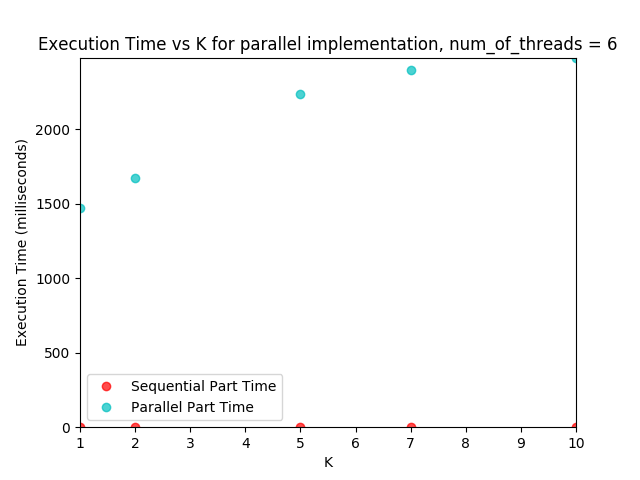
\includegraphics[width=\linewidth]{assets/time_vs_K_parallel_num_of_threads_6.png}
\label{fig:test1}
\vspace{-2pt}
\caption{Execution time vs K for parallel implementation. num\_of\_threads is set to 6.}
\end{figure}
\subsubsection{Discussion}
\qquad From the plot, we can infer that the running time of the parallel implementation also depends on the value of k. As the value of k increases, parallel running time increases since computation per thread increases.

\subsubsection{Sequential Implementation}
\begin{figure}[H]
\centering
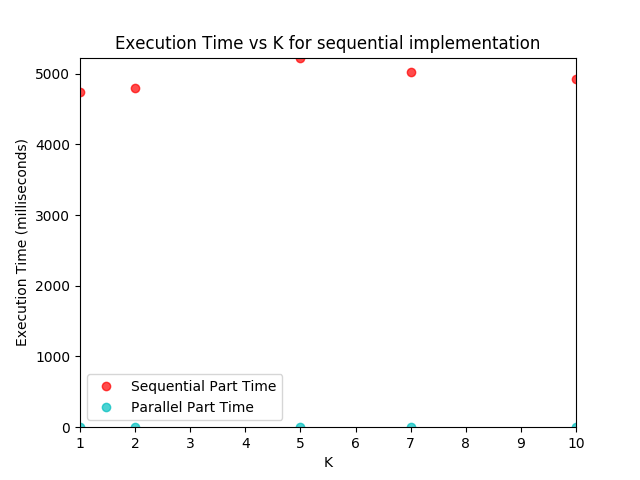
\includegraphics[width=\linewidth]{assets/time_vs_K_sequential.png}
\label{fig:test1}
\vspace{-2pt}
\caption{Execution time vs K for sequential implementation.}
\end{figure}

\subsubsection{Discussion}
\qquad From the plot we can infer that sequential time still increases with respect to the K value but the increase is not as drastic as parallel implementation. This is because as K increases training set size increases but test set size decreases. Hence the total number of images stay the same. Histograms of both training set and test set are computed. For lower K values, larger number of test set examples are compared(computed distance between a training set image and test set image) with smaller number of training set examples. For higher K values, smaller number of test set examples are compared with larger number of training set examples. Hence in both cases total computation is similar to each other. The changes in the results for different K values is due to the current state of the computer where the code is executed on. On the other hand parallel runtime is always 0 because sequential implementation does not have a parallel part.


\subsection{Profiling Outputs Using gprof}
\qquad The following analysis is based on the previously generated prof\_sequential.txt and prof\_omp.txt files.
\subsubsection{Sequential Implementation}
\qquad  By investigating the flat profile for sequential program, we see that create\_histogram function contributes 70\% of the total runtime, distance function contributes 14.93\% and read\_pgm\_file function also contributes 14.93\% percent of the total running time. The other functions also contribute to the total runtime as well but they are not influential as the mentioned functions. This \%time analysis shows that the main bottleneck of the sequential implementation are calls to create\_histogram, distance and read\_pgm\_file functions. Therefore, the flat profile shows that it would be meaningful to parallelize these portions of the implementation to make this code faster. Note that distance function generates its portion of running time through the calls from find\_closest to it(this will be more apparent in the call graph analysis). Also by looking to the self field, we see that create\_histogram takes 0.47 seconds(the most time consuming), read\_pgm\_file and distance functions take 0.10 seconds each. Other functions also consume time it appears that the most influential(bottleneck) functions are the mentioned. The calls field shows that distance function is called 32400 times, create\_histogram and read\_pgm\_file functions are called 360 times each. In like manner, by looking at the calls and self field of the flat profile, we see that it meaningful to parallelize create\_histogram and distance functions. Note that read\_pgm\_file function is given in the util file so it is not attempted to be parallelized. \\
\null \qquad By investigating Call Graph for the sequential program, we see that main and its descendants contribute 100\% to the total running time. This is meaningful since  the main function is run in C  by default. create\_histogram function and its descendants contribute 70\% to the total running time. Since the percentage of contribution is same for create\_histogram function in both call graph and flat profile, create histogram should not do a significant job by calling another declared function. This is indeed the case with the create\_histogram function. A similar inference can be done for distance and read\_pgm\_file functions. On the other hand, 14.9\% contribution from find\_closest function and its distance is due to the distance function calls in find\_closest function. In fact, the distance function is only called in find\_closest function. 

\subsubsection{Parallel Implementation}
\qquad By investigating the flat profile and call graph together, we see that compared to the sequential program, there is a different result in terms of time proportional division to the functions. According to the profiling outputs for different threads for K = 10, main function and read\_pgm\_file functions contribute most to the total time. But this should not be the case. After a research on using gprof with multithreaded programs, I found out that gprof only profiles the main thread but not the threads created by OpenMP. Therefore, we can not infer a correct conclusion from these results. For example, create\_histogram function did the most job in sequential implementation however, it is listed as 0 in all of the parallel profiling results. The two explanations for this results is that either the sequential implementation is parallelized in a good proportion or the main thread only runs read\_pgm\_file function. In conclusion, gprof is not suitable for multi-threaded program profiling and a more sophisticated profiler should be used.

\end{document}